%% Box 1 — Megaprojects capex comparison and its limits

\begin{fullwidth}
\begin{tcolorbox}[datacenterbox,
  title={Box 1\enspace Data centers as a megaproject? Scale, comparability, and the limits of the analogy}]

\begin{minipage}[t]{\linewidth}
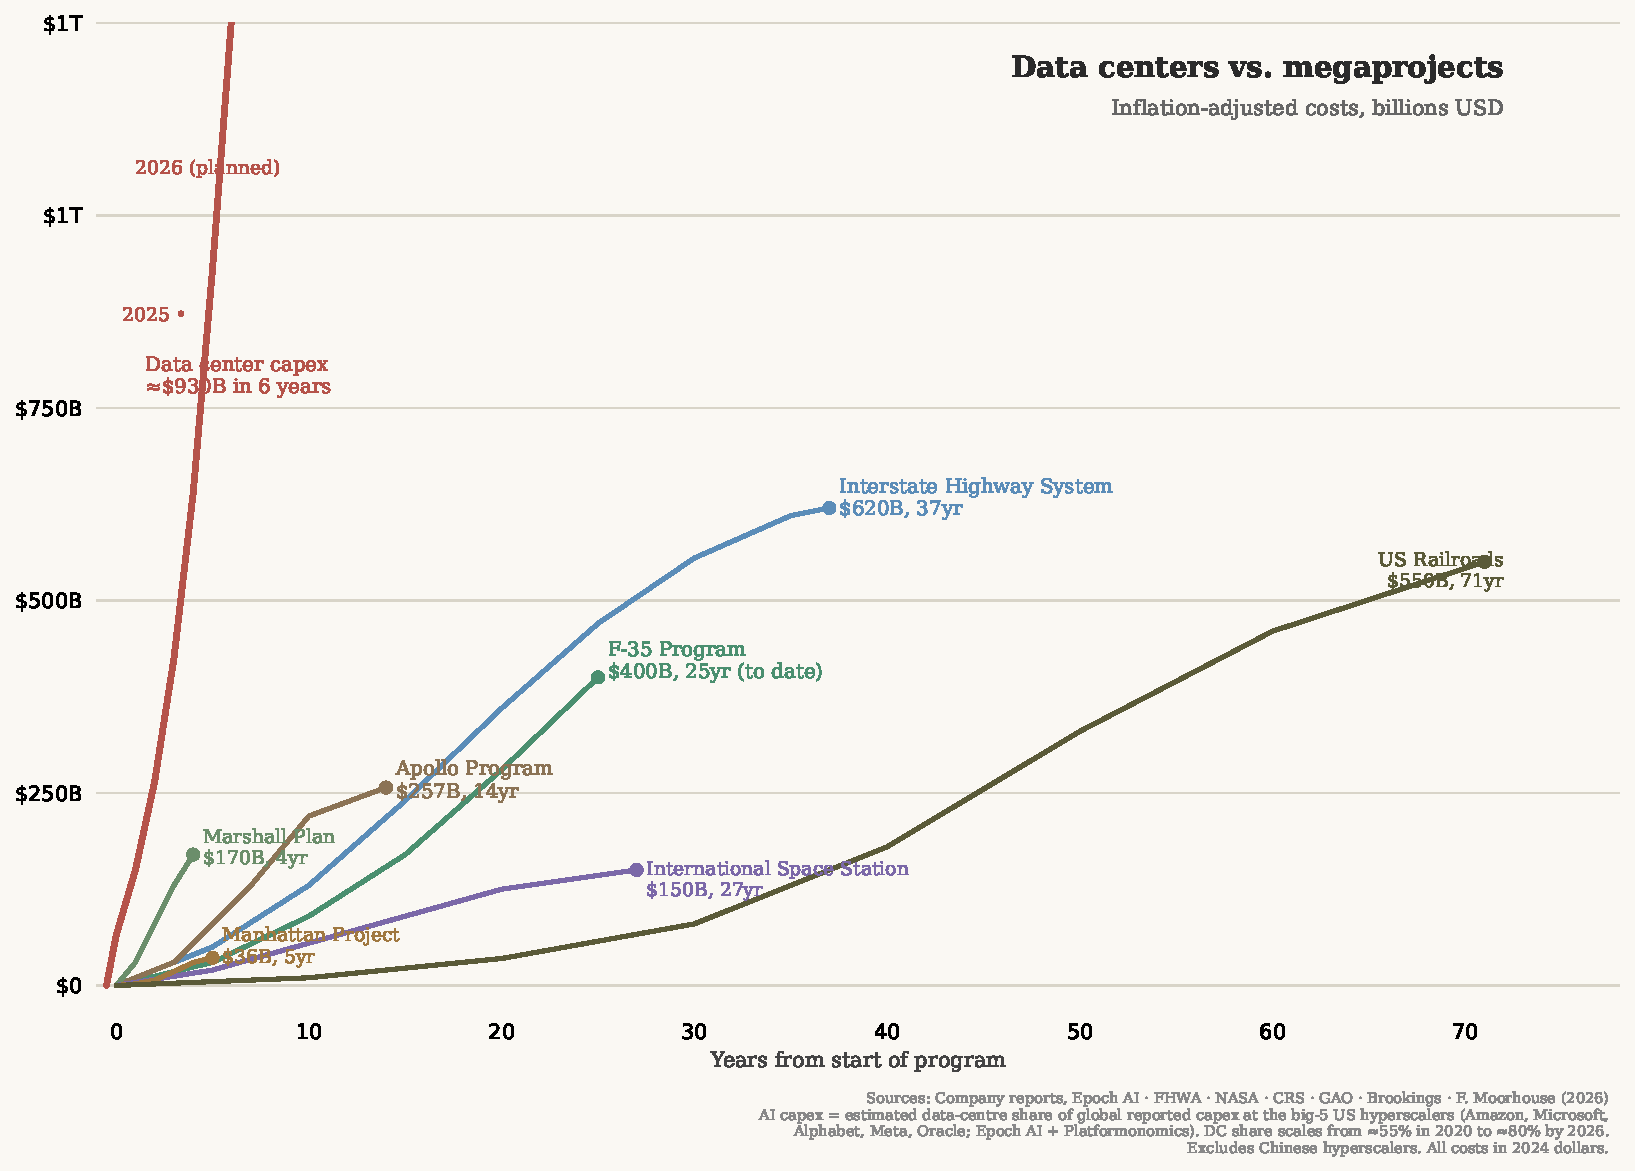
\includegraphics[width=\linewidth]{figures/megaprojects_capex}
\vspace{0.3em}
{\footnotesize\textit{Figure.} Cumulative data center capex (2019--2025, projected 2026) against
historical megaprojects, inflation-adjusted 2024 USD. Data: Epoch AI / Platformonomics;
FHWA; NASA; CRS; GAO; Brookings. Chart style after \citet{moorhouse2026megaprojects}.
All costs in 2024 dollars; Chinese hyperscalers excluded.}
\end{minipage}

\smallskip\noindent\rule{\linewidth}{0.3pt}\smallskip

\noindent\textbf{Why the comparison is powerful — and why it is also misleading.}\enspace
The chart circulates widely as evidence that data center investment has become the
defining infrastructure programme of the present moment, surpassing in speed and
aggregate cost anything the public sector has attempted since the Interstate Highway
System. As a rhetorical device it works: the visual comparison compresses the argument
into a single image.

As an analytical claim, however, the comparison conflates incommensurable categories.
\textit{First}, private recurring capital expenditure — distributed across thousands of
facilities, operators, and jurisdictions, repaid through commercial returns — is
structurally different from one-off public programmes underwritten by sovereign credit
and motivated by collective goods. The Apollo Programme produced the Moon landing and
was then wound down; data center capex is an indefinitely renewing operational
commitment whose cumulative figure grows by definition every year.
\textit{Second}, the comparison exploits the asymmetry of cumulation: summing six years
of annual private capex and setting it against the total lifetime cost of a 37-year
programme makes the former appear commensurately large, but the correct comparison is
the annual \textit{rate} of investment — at which point the Interstate Highway System
absorbed a larger share of US GDP for longer than the current data center build-out.
\textit{Third}, the data center capex figure rests on an opaque imputation methodology
(a DC share of hyperscaler capex scaling from $\approx$55\% to $\approx$80% across
the period) that is not independently verifiable and excludes Chinese hyperscalers
whose inclusion would substantially alter the comparison.
\textit{Fourth}, the selection of comparators does rhetorical work: there is no
equivalent chart for telecoms network buildout (1990--2000), rural electrification
(1935--1950), or the transatlantic cable system — all of which would likely produce
similar or larger figures on the same axes.

The chart is cited here not as authoritative evidence of scale but as a data point
about the \textit{genre of claim} being made about data centers in public discourse.
The fact that this particular comparison circulates as widely as it does — through
Epoch AI reports, policy briefs, and social media — is itself a finding: it indicates
that the governance and accountability frameworks for data center infrastructure are
being formed in an environment where the dominant reference points are wartime
mobilisation and Cold War programmes, not the regulatory regimes developed for
utilities, telecommunications, or land-use planning. The analogy shapes what
interventions appear plausible.

\end{tcolorbox}
\end{fullwidth}
